\documentclass{ntuthesis}

\usepackage{times}
\usepackage{verbatim}
\usepackage{color}
\usepackage{url}
\usepackage{graphicx} %Loading the package
\usepackage{caption}
\usepackage{subcaption}
\usepackage[export]{adjustbox}
\graphicspath{
    {img/}
    {img/VanishingComp/}
    {img/Sec3/sim1/}
    {img/Sec4/sim1/}
    {img/Sec4/sim2/}
    {img/Sec4/sim3/}
    {img/Sec5/sim1/}
    {img/Sec5/sim2/}
    {img/Sec6/sim1/}
    {img/Sec6/theo1/}
    {img/Simulation/}
    {img/supp/}
}
\usepackage{array}
\usepackage{wallpaper}
\usepackage{hyperref}

\usepackage{booktabs}       % professional-quality tables
\usepackage{amsfonts}       % blackboard math symbols
\usepackage{nicefrac}       % compact symbols for 1/2, etc.
\usepackage{microtype}      % microtypography
\usepackage{multirow}

\usepackage{times}
\usepackage{helvet}
\usepackage{courier}
\usepackage{amsmath}
\usepackage{tikz}
\usepackage{array}
\usepackage{makecell}
\renewcommand{\cellalign}{cc}

\usepackage{letltxmacro}
\LetLtxMacro{\originaleqref}{\eqref}
\renewcommand{\eqref}{eqn.~\originaleqref}

\usepackage[printwatermark]{xwatermark}
\usepackage{pdfpages}

% Using the tex-text mapping for ligatures etc.
\defaultfontfeatures{Mapping=tex-text}

% Set the default fonts
\setmainfont{Times New Roman}
\setCJKmainfont{標楷體}

\ifdefined\withwatermark
  \newwatermark*[allpages,xpos=6.1725cm,ypos=10.5225cm,scale=0.5]{\includegraphics{watermark.pdf}}
\fi

% digital object identifier
\ifdefined\withdoi
  \insertdoi
\fi

\makeatletter
\AtBeginDocument{
  \hypersetup{
    pdftitle={\@titleen},
    pdfauthor={\@authoren},
    pdfsubject={\@typeen{} \@classen},
    pdfkeywords={\@keywordsen}
  }
}
\makeatother

% Your information goes here
% author: Tz-Huan Huang [http://www.csie.ntu.edu.tw/~tzhuan]

% ----------------------------------------------------------------------------
% "THE CHOCOLATE-WARE LICENSE":
% Tz-Huan Huang wrote this file. As long as you retain this notice you
% can do whatever you want with this stuff. If we meet some day, and you think
% this stuff is worth it, you can buy me a chocolate in return Tz-Huan Huang
% ----------------------------------------------------------------------------

% Syntax: \var{English}{Chinese}
\university{National Taiwan University}{國立臺灣大學}
\college{College of Electrical Engineering and Computer Science}{電機資訊學院}
\institute{Graduate Institute of Communication Engineering}{電信工程學研究所}
\title{Vanishing Nodes: Another Phenomena That Makes Training Deep Neural Networks Difficult}
{神經元消失:使深層神經網路難以訓練的另一種現象}
\author{Wen-Yu Chang}{張文于}
\studentid{R06942064}
\advisor{Tsung-Nan Lin}{林宗男}
\defenseyear{2019}{108}
\defensemonth{July}{7}
\defenseday{8}
\doi{doi:}
\keywords{Deep learning, Vanishing gradient, Learning theory}{深度學習, 梯度消失, 機器學習理論}


\begin{document}

\frontmatter

\makecover

% \ifdefined\withcertification
%   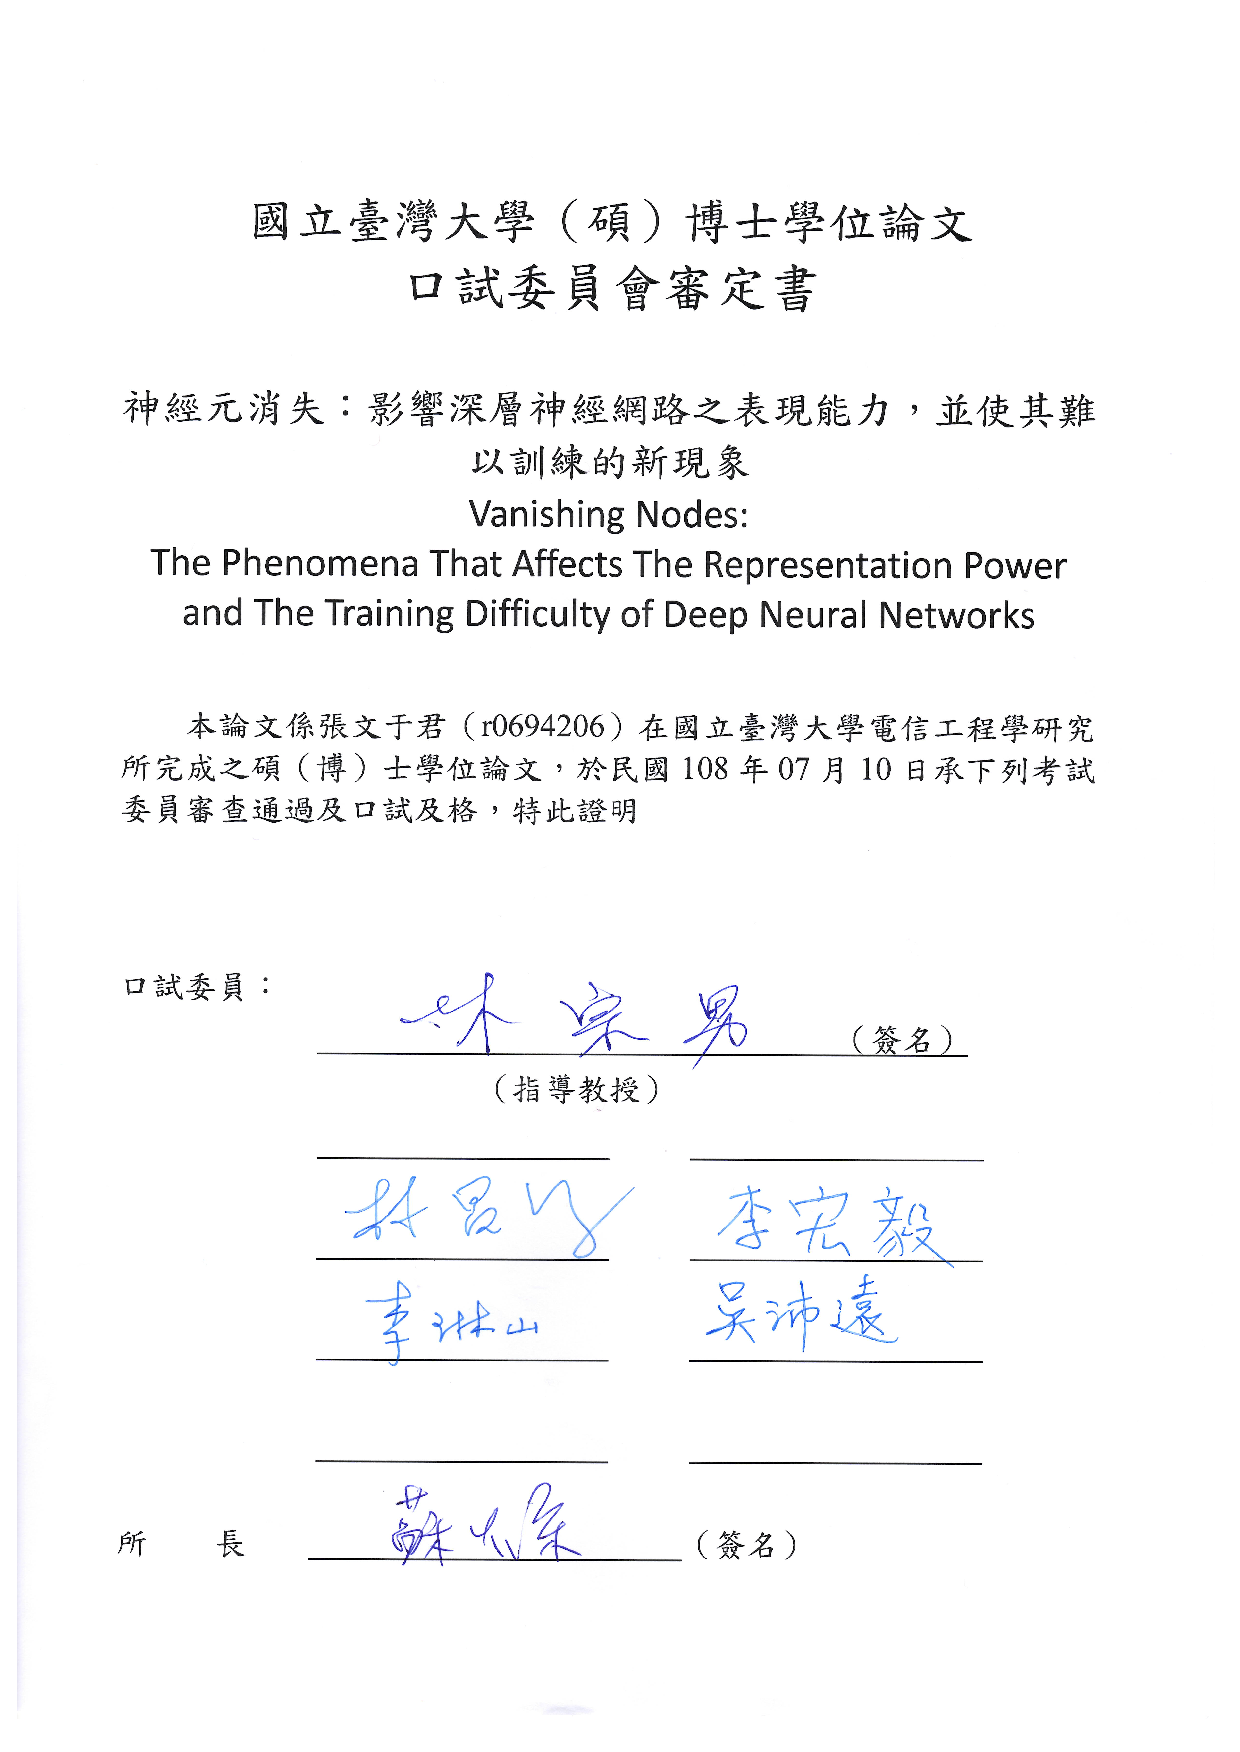
\includepdf[angle=0]{certification.pdf}
% \else
%   \makecertification
% \fi

% \input{acknowledgements}
\begin{abstractzh}
    梯度爆炸/消失,一直被認為是訓練深層神經網路的一大挑戰。
    在這篇論文裡,我們發現一種被稱為
    「神經元消失 (Vanishing Nodes)」
    的新現象同樣也會使訓練更加困難。
    當神經網路的深度增加,神經元彼此之間的會呈現高度相關。
    這種行為會導致神經元之間的相似程度提高。
    也就是隨著神經網路變深,網路內的神經元冗餘程度會提高。
    我們把這個問題稱為「神經元消失 (Vanishing Nodes)」。
    可以藉由神經網路的相關參數來對神經元消失的程度做推算;
    結果可以得出神經元消失的程度與網路深度成正比、與網路寬度成反比。
    從數值分析的結果呈現出:在反向傳播算法的訓練下,
    神經元消失的現象會變得更明顯。
    我們也提出:神經元消失是除了梯度爆炸/消失以外,
    訓練深層神經網路的另一道難關。

\bigbreak
\noindent \textbf{關鍵字:}{\, \makeatletter \@keywordszh \makeatother}
\end{abstractzh}

\begin{abstracten}
    It is well known that the problem of vanishing/exploding gradients creates a challenge when 
    training deep networks. In this paper, we show another phenomenon, called \textit{vanishing nodes},
    that also increases the difficulty of training deep neural networks.
    As the depth of a neural network increases, the network's hidden nodes show more highly
    correlated behavior. This correlated behavior results in great similarity between these nodes.
    The redundancy of hidden nodes thus increases as the network becomes deeper.
    We call this problem "\textit{Vanishing Nodes}."
    This behavior of vanishing nodes can be characterized quantitatively by the network parameters,
    which is shown analytically to be proportional to the network depth and inversely proportional
    to the network width. The numerical results suggest that the degree of vanishing nodes will become
    more evident during back-propagation training. Finally, we show that vanishing/exploding gradients
    and vanishing nodes are two different challenges that increase the difficulty of training deep
    neural networks.

\bigbreak
\noindent \textbf{Keywords:}{\, \makeatletter \@keywordsen \makeatother}
\end{abstracten}

\begin{comment}
\category{I2.10}{Computing Methodologies}{Artificial Intelligence --
Vision and Scene Understanding} \category{H5.3}{Information
Systems}{Information Interfaces and Presentation (HCI) -- Web-based
Interaction.}

\terms{Design, Human factors, Performance.}

\keywords{Deep learning}
\end{comment}


\tableofcontents
\listoffigures
\listoftables

\mainmatter

% Your thesis goes here
\chapter{Introduction}
\label{c:intro}

Deep neural networks (DNN) have succeeded in various fields, including computer vision \cite{alexnet}, speech recognition \cite{speech}, machine translation \cite{google_trans}, medical analysis \cite{medical} and human games \cite{alphago}. Some results are comparable to or even better than those of human experts.


State-of-the-art methods in many tasks have recently used increasingly \textit{deep} neural network architectures. The performance has improved as networks have been made \textit{deeper}. For example, some of the best-performing models \cite{resnet1, resnet2} in computer vision have included hundreds of layers.

Moreover, recent studies have found that as the depth of a neural network increases, problems such as vanishing or exploding gradients make the training process more challenging. \cite{xavier, he} investigated this problem deeply and suggested that initializing weights in appropriate scales can prevent gradients from vanishing or exploding exponentially.
\cite{mft:expo, mft:info} also studied how vanishing/exploding gradients arise via \textit{mean field theory} and provided a solid theoretical discriminant to determine whether the propagation of gradients is vanishing/exploding. 

Inspired by previous studies, we investigated the correlation between hidden nodes and discovered that a phenomenon that we call \textit{vanishing nodes} can also affect the capability of a neural network.
In general, the hidden nodes of a neural network become highly correlated as the network becomes deeper.
The correlation between nodes implies the similarity between them, and high degree of similarity between nodes produces redundancy.
Because a sufficient number of effective nodes is needed to approximate an arbitrary function, the redundancy of nodes in hidden layers may debilitate the representation capability of the entire network.
Thus, as the depth of the network increases, the redundancy of hidden nodes may increase and hence affect the network's trainability. We name this phenomena as "\textit{Vanishing Nodes}."

We propose a \textit{Vanishing Node Indicator (VNI)}, which is the weighted average of squared correlation coefficients, as the quantitative metric for vanishing nodes. VNI can be theoretically approximated via the results on the spectral density of the end-to-end Jacobian. The approximation of  VNI depends on the network parameters, including the width, the depth, the distribution of weights, and the activation functions, and it is shown to be simply proportional to the network depth and inversely proportional to the network width.

In addition, the numerical results show that back-propagation training also intensifies the correlations of hidden nodes when we consider a deep network.
We find that although we use a relatively large network width, the correlations of hidden nodes may still increase during the training process.

%Finally, we show that vanishing/exploding gradients and vanishing nodes are two different problems, so the two problems may arise from certain conditions respectively. We provide a criterion to predict the occurrences of two problems via parameters of the network setting including the network depth, the network width, the activation function and the weight initialization. That is, our criterion is widely applicable for various neural network architectures.

% In recent years, mean field theory and dynamical isometry have been used for theoretical analysis of DNN. The related works \cite{mft:sigmoid, mft:spectral} have give mathematical predictions which are excellent agree with the empirical result on vanishing/exploding gradients. Moreover, it addressed that preserving the norms of gradients, i.e. making the mean squared singular value of a network’s input-output Jacobian close to 1, is \textit{necessary} but not \textit{sufficient} condition for achieving dynamical isometry. An analysis on deep linear network \cite{mft:linear} has shown that network initializations satisfying dynamical isometry yield a faster learning speed compared to initializations that do not. Several works also observed that dynamical isometry is important for ensuring the \textit{trainability} of deep feed-forward networks \cite{mft:sigmoid, mft:spectral}, deep convolutional neural networks(CNN) \cite{mft:cnn}, and even recurrent neural networks(RNN) \cite{mft:rnn}.

% However, we are curious about the cause of the ill-training situation when dynamical isometry is not satisfied. We observed that in a failed training of a DNN, after several training batches, activation values and gradients of many neurons are highly-correlated. We call it \textit{Resonance Phenomena}. We found that the occurrence of this phenomena makes the training process more difficult. Moreover, the phenomena occurs even if the norms of gradients are preserved.


% We found that orthogonal weight initialization or residual shortcut will reduce the resonance phenomena. In this paper, we also proposed another solution to reduce the resonance phenomena.

%In the body of this paper, we provide some related works in Section \ref{related}, discuss the importance of the correlation of hidden nodes and give both theoretical analysis and results of numerical simulation on the vanishing nodes phenomena in Section \ref{why}, compare the vanishing nodes problem with vanishing/exploding gradients in Section \ref{compare}, and make the conclusion in Section \ref{conclusion}.

Finally, we show that vanishing/exploding gradients and vanishing nodes are two different problems, so that the two problems may arise from specific conditions. The experimental results show that the likelihood of failed training increases as the depth of the network increases. The training will become much more difficult due to lack of network representation capability. 

This paper is organized as follows: some related works are discussed in Section \ref{related}. The vanishing nodes phenomenon is introduced in Section \ref{why}. Theoretical analysis and a quantitative metric are  reported in Section \ref{why}. Section \ref{compare} compares the vanishing nodes with vanishing/exploding gradients. Section \ref{experiments} reports the experimental results and Section \ref{conclusion} gives our conclusions.


\chapter{Related Work}
\label{related}

Problems in the training of deep neural networks have been encountered in several studies.
For example, \cite{xavier, he} investigated vanishing/exploding gradient propagation and gave weight initialization methods as the solution. \cite{evop} suggested that vanishing/exploding gradients might relate to the sum of the reciprocals of the hidden layer widths.
\cite{opt_prob, saddle} stated that saddle points are more likely than local minima to be a problem for training deep neural networks.
\cite{degrade1, degrade2, resnet1} exposed the \textit{degradation} problem: the performance of a deep neural network degrades as the depth increases.

The correlation between the nodes of hidden layers within a deep neural network is the main focus of this paper, and several kinds of correlations have been discussed in the literature.
%, while several kinds of correlations have been discussed. In this work, we proposed a different problem related to the correlation between two nodes in a hidden layer.
\cite{mft:info} surveyed the propagation of the correlation between two different inputs after several layers.
\cite{whiten1, whiten2} suggested that the input features must be whitened (i.e., zero-mean, unit variances and uncorrelated) to achieve a faster training speed.

Dynamical isometry is one of the conditions that make ultra-deep network training more feasible.
\cite{mft:linear} reported dynamical isometry to theoretically ensure depth-independent learning speed.
\cite{mft:sigmoid, mft:spectral} suggested several ways to achieve dynamical isometry for various settings of network architecture, and \cite{mft:cnn, mft:rnn} practically trained ultra-deep networks in various tasks.

\chapter{Vanishing Nodes: correlation between hidden nodes}
\label{why}

In this section, the correlation of hidden-layer neurons is investigated.
If a pair of neurons is highly correlated (for example, the correlation coefficient is equal to $+1$ or $-1$), one of the neurons becomes redundant.
Great similarity between nodes may reduce the effective number of neurons within a network.
In some cases, the correlation of hidden nodes may disable the entire network. This phenomenon is called \textit{Vanishing Nodes}.

% In this section, we would like to show the importance of correlation of hidden layer nodes.
% We will define the correlation metric, show that the highly correlated hidden nodes may reduce the effective width of a neural network, and then connect the width of a network to its representation capability.
% We find that in some cases, the correlation of hidden nodes in a network may disable the whole network.
% We name this phenomena as \textit{vanishing nodes}, and we provide an intuitive example to demonstrate it.

First, consider a deep feed-forward neural network with depth $L$.
For simplicity of analysis, we assume all layers have the same width $N$.
The weight matrix of layer $l$ is $\mathbf{W}_l\in \mathbb{R}^{N\times N}$, the bias of layer $l$ is $\mathbf{b}_l\in \mathbb{R}^N$ (a column vector), and the common activation function of all layers is $\phi(\cdot):\mathbb{R}\rightarrow \mathbb{R}$. The input of the network is $\mathbf{x}_0$, and the nodes at output layer $L$ denote $\mathbf{x}_L$. The pre-activation of layer $l$ is $\mathbf{h}_l\in \mathbb{R}^N$ (a column vector), and the post-activation of layer $l$ is $\mathbf{x}_l\in \mathbb{R}^N$ (a column vector). That is, $\forall l \in \{1, ..., L\}$,

\begin{equation}
    \mathbf{h}_l=\mathbf{W}_l\mathbf{x}_{l-1}+\mathbf{b}_l,\;\;\;
    \mathbf{x}_{l}=\phi(\mathbf{h}_l).
\label{network_eqn}
\end{equation}

The variance of node $i$ is defined as $\sigma_i^2\overset{\Delta}{=}\mathbb{E}_{\mathbf{x}_0}[(x_{l(i)}-\overline{x_{l(i)}})^2]$, and the squared correlation coefficient ($\rho_{ij}^2$) between nodes $i$ and $j$ can be computed as $\rho_{ij}^2\overset{\Delta}{=}
\frac
{\mathbb{E}_{\mathbf{x}_0}[(x_{l(i)}-\overline{x_{l(i)}})(x_{l(j)}-\overline{x_{l(j)}})]^2}
{\mathbb{E}_{\mathbf{x}_0}[(x_{l(i)}-\overline{x_{l(i)}})^2]\mathbb{E}_{\mathbf{x}_0}[(x_{l(j)}-\overline{x_{l(j)}})^2]},$
where $\rho_{ij}^2$ ranges from $0$ to $1$.
Nodes $x_{l(i)}$ and $x_{l(j)}$ are highly correlated only if the magnitude of the correlation coefficient between two nodes $\rho_{ij}$ is nearly 1. $\rho_{ij}^2$ indicates the magnitude of similarity between node $i$ and node $j$.
If $\rho_{ij}$ is close to $+1$ or $-1$, then node $i$ can be approximated in a linear fashion by node $j$. Great similarity indicates redundancy. If nodes of hidden layers exhibit great similarity, the effective number of nodes will be much lower than the original network width. Therefore, we call this phenomena \textit{Vanishing Node Problem}.



%Recent works have put emphasis on the depth of a neural network, since the \textit{width} of a neural network also matters.
%According to the "universal approximation theorem" proved by \cite{universal}, a single hidden layer with a finite number of neurons can approximate continuous functions on compact subsets.
%That is, the number of neurons in a network is closely related to its representation power, which is .

%Vanishing node is a problem that in some cases, several nodes in hidden layers or the output layer in a neural network architecture are highly correlated even if nodes of the input layer are independent.
%Correlations imply dependencies, and dependencies produce redundancy.
%That is, in the worst case, all of hidden nodes or output nodes are so correlated that if we remove the redundant nodes, the number of remaining nodes are much less than the original network width.
%Therefore, we name this phenomena as the \textit{vanishing node problem}.

% \begin{figure}
    \begin{minipage}[c]{0.4\textwidth}
        \caption{We use the product of many Gaussian-initialized matrices as our \textit{"correlated-initialized"} weight matrix. To show the levels of correlation versus the number of matrices in the product, we plot the averaged cosine similarities of weight vectors. Notice that the number of nodes $N$ in hidden layers are all 6.}
        \label{fig:sec3_sim1}
    \end{minipage}\hfill
    \begin{minipage}[c]{0.5\textwidth}
        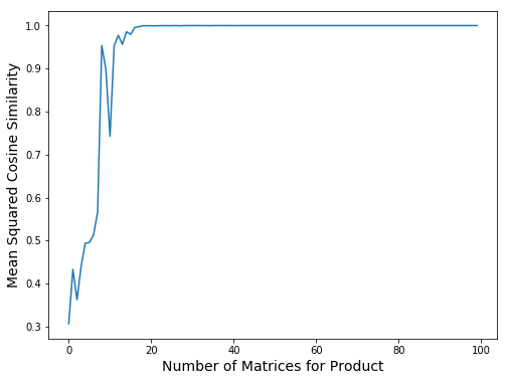
\includegraphics[width=\textwidth]{CorrelatedInitialization}
    \end{minipage}
\end{figure}

%\section{Results} \label{results}

In the following section, we propose a metric to measure the quantitative property of vanishing nodes for a deep feed-forward neural network.
Theoretical analysis of the metric indicates that the quantitative property of vanishing nodes is proportional to the network depth and inversely proportional to the network width.
The quantity is shown analytically to depend on the statistical property of weights and the nonlinear activation function. 

% In this section, we will (1) provide a theoretical analysis on the accumulation of the node correlation just after the weight initialization (2) give a numerical results for presenting that the weights update via back-propagation will intensify the node correlation.

%\section{Network Depth Makes Initial Correlations Accumulate} \label{initial}
\section{Vanishing Node Indicator} \label{initial}

Consider the network architecture defined in \eqref{network_eqn}. In addition, the following assumptions are made: (1) The input $\mathbf{x}_0$ is zero-mean, and the features in $\mathbf{x}_0$ are independent and identically distributed. (2) All weight matrices $\mathbf{W}_l$ in each layer are initialized from the same distribution with variance $\sigma_w^2/N$. (3) All the bias vectors $\mathbf{b}_l$ in each layer are initialized to zero.
% We would like to provide an analysis on the correlation of output nodes in a deep neural network. We will first setup a network, define a metric for measuring the correlation, perform theoretical analysis on the metric, and then provide several results of numerical simulations.

% To analyze the correlation of output layer nodes toward depth, we need to define a metric to measure the output layer node correlation.
% First, consider the network architecture we defined in \eqref{network_eqn}.
% In particular, we have made several assumptions: (1) The input $\mathbf{x}_0$ is zero-mean, and features in $\mathbf{x}_0$ are independent and identically distributed. (2) All the weight matrices $\mathbf{W}_l$ in each layer are initialized from a same distribution with variance $\sigma_w^2/N$. (3) All the bias vectors $\mathbf{b}_l$ in each layer are initialized to zero.

The input-output Jacobian matrix $\mathbf{J}\in\mathbb{R}^{N\times N}$  is defined as the first-order partial derivative of the output layer with respect to the input layer, which can be rewritten as $\frac{\partial\mathbf{x}_L}{\partial\mathbf{x}_0}=\prod_{l=1}^{L}\mathbf{D}_l\mathbf{W}_l$,
where $\mathbf{D}_l\overset{\Delta}{=} diag(\phi'(\mathbf{h}_l))$ is the derivative of point-wise activation function $\phi$ at layer $l$.
% With the input-output Jacobian and the given assumptions, we can perform the first-order forward approximation:
To conduct a similar analysis as \cite{mft:linear}, consider the first-order forward approximation:
$\mathbf{x}_L-\overline{\mathbf{x}_L} \approx \mathbf{Jx}_0$. Therefore, the covariance matrix of the nodes ($\mathbf{C}\in\mathbb{R}^{N\times N}$) at the output layer  can be computed as

\begin{equation}
    \mathbf{C} \overset{\Delta}{=}
    \mathbb{E}_{\mathbf{x}_0}[(\mathbf{x}_L-\overline{\mathbf{x}_L})(\mathbf{x}_L-\overline{\mathbf{x}_L})^T]
    \approx
    \mathbb{E}_{\mathbf{x}_0}[(\mathbf{Jx}_0)(\mathbf{Jx}_0)^T]
    =
    \mathbf{J}\mathbb{E}_{\mathbf{x}_0}[\mathbf{x}_0\mathbf{x}_0^T]\mathbf{J}^T
    =
    \sigma_x^2\mathbf{J}\mathbf{J}^T,
    \label{covariance_eqn}
\end{equation}

where $\sigma_x^2$ is the common variance of features in $\mathbf{x}_0$, and the expected values are calculated with respect to the input $\mathbf{x}_0$. For notational simplicity, we omit the subscript $\mathbf{x}_0$ of the expectations in the following equations. 
It can be easily derived that the squared covariance of nodes $i$ and $j$ is equal to the product of the squared correlation coefficient and the two variances. That is, $[C_{(ij)}]^2=\rho_{ij}^2\sigma_i^2\sigma_j^2$.

In this paper, we propose the \textit{Vanishing Node Indicator (VNI)} $R_{sq}$ to quantitatively characterize the degree of vanishing nodes for a given network architecture. It is defined as follows:

\begin{equation}
    R_{sq}\overset{\Delta}{=}
    \frac{\sum_{i=1}^N\sum_{j=1}^N\rho_{ij}^2\sigma_i^2\sigma_j^2}
{\sum_{i=1}^N\sum_{j=1}^N\sigma_i^2\sigma_j^2}.
\label{rsq_def}
\end{equation}

VNI calculates the weighted average of the squared correlation coefficients $\rho_{ij}^2$ between output layer nodes with non-negative weights $\sigma_i^2\sigma_j^2$. Basically, VNI $R_{sq}$, which ranges from $1/N$ to $1$, summarizes the similarity of the nodes at the output layer. If all nodes are independent of each other, the correlation coefficients $\rho_{ij}$ will be 0 (if $i\neq j$) or 1 (if $i=j$) and $R_{sq}$ will become the minimum value of $1/N$.
Otherwise, if all of the output nodes are highly correlated, then all squared correlation coefficients $\rho_{ij}^2$ will be nearly 1, and therefore $R_{sq}$ will reach the maximum value of $1$.
Note that the weights $\sigma_i^2\sigma_j^2$ in the weighted average can be interpreted as the importance of the output-layer nodes $i$ and $j$. If all of the output layer nodes have equal variances, VNI $R_{sq}$ is simply reduced to the average of the squared correlation coefficients $\rho_{ij}^2$.


\begin{figure}[h]
\centering
\newcommand{\myWidth}{0.48\textwidth}
\begin{subfigure}{\myWidth}
  \centering
  \caption{Network width $N=200$}
  \includegraphics[width=1.0\linewidth,trim={0 0 0 0.8cm},clip]{"MNIST_TanhWidth200(059)"}
  \label{fig:sec4_sim2_a}
\end{subfigure}

\begin{subfigure}{\myWidth}
  \centering
  \caption{Network width $N=500$}
  \includegraphics[width=1.0\linewidth,trim={0 0 0 0.8cm},clip]{"MNIST_TanhWidth500(059)"}
  \label{fig:sec4_sim2_b}
\end{subfigure}%

\caption{
The results of VNI $R_{sq}$ with respect to network depth $L$ for the network width 200 and 500. The red line is calculated from \eqref{rsq_moment}, the blue line is computed from \eqref{rsq_def} with the input data of zero mean and i.i.d input data, and the green line is computed from \eqref{rsq_def} with MNIST data.
%from theoretical analysis (red), simulation with i.i.d. inputs (blue) and simulation with MNIST inputs (green).
The VNI $R_{sq}$ expressed in \eqref{rsq_moment} is very close to the original definition in \eqref{rsq_def}.
% Note that the theoretical value of VNI is $R_{sq}\approx\frac{1}{N}\Big(\frac{L}{0.998}+1\Big)$ for the scaled-Gaussian weight  initialization ($s_1=-1$) and the $Hard\text{-}Tanh$ activation ($\mu_k=erf\big(\frac{1}{\sqrt{2\cdot 0.1}}\big)$).
}
\label{fig:sec4_sim2}
\end{figure}


With the covariance matrix defined in \eqref{covariance_eqn} and the formulas for matrix traces, VNI $R_{sq}$ can be expressed as the formula of the covariance matrix as
\begin{equation}
    \begin{aligned}
    R_{sq}
    &=\frac{
    \sum_{i=1}^N\sum_{j=1}^N\mathbb{E}_{\mathbf{x}_0}
    [(x_{L(i)}-\overline{x_{L(i)}})(x_{L(j)}-\overline{x_{L(j)}})]^2
    }{
    \sum_{i=1}^N\sum_{j=1}^N
    \mathbb{E}_{\mathbf{x}_0}[(x_{L(i)}-\overline{x_{L(i)}})^2]
    \mathbb{E}[(x_{L(j)}-\overline{x_{L(j)}})^2]
    }\\
    &=
    \frac{\sum_{i=1}^N\sum_{j=1}^N[C_{(ij)}]^2}
    {\sum_{i=1}^N\sum_{j=1}^NC_{(ii)}C_{(jj)}}
    =
    \frac{tr(\mathbf{C}{\mathbf{C}}^T)}
    {tr(\mathbf{C})^2}
    ,
    \end{aligned}
    \label{rsq_eqn}
\end{equation}
where $tr(\cdot)$ is the matrix trace operation.

From \eqref{covariance_eqn}, substituting $\sigma_x^2\mathbf{JJ}^T$ for $\mathbf{C}$ in \eqref{rsq_eqn}, and noting that $tr(\mathbf{A}^k)$ is equal to the sum of eigenvalues to the $k$-th power of symmetric matrix $\mathbf{A}$ \cite{matrix}, an approximation of $R_{sq}$ can be obtained:

\begin{equation}
    R_{sq}\approx
    \frac{tr(\mathbf{JJ}^T\mathbf{JJ}^T)}{tr(\mathbf{JJ}^T)^2}
    =\frac{\sum_{k=1}^N\lambda_k^2}{(\sum_{k=1}^N\lambda_k)^2}
    =\frac{N\cdot m_2}{(N\cdot m_1)^2}
    =\frac{m_2}{Nm_1^2},
    \label{rsq_eigen}
\end{equation}

where $\lambda_k$ is the $k$-th eigenvalue of $\mathbf{JJ}^T$, and $m_i$ is the $i$-th moment of eigenvalues of $\mathbf{JJ}^T$.

%In \eqref{rsq_eigen}, we show that  $R_{sq}$ is related to the moments of eigenvalues of $\mathbf{JJ}^T$. Since the moments of eigenvalues of $\mathbf{JJ}^T$ have been analyzed in previous work (\cite{mft:spectral},) we would like to insert the result for the moments of eigenvalues, which is related to the network depth $L$, the network width $N$, the activation function $\phi(\cdot)$ and weight initialization, into the approximation of $R_{sq}$.

%For simplicity, let's assume that the weights of all layers $\mathbf{W}_l$ share a common distribution as $\mathbf{W}$. Also, assume the variances of all hidden layers are the same, which implies the $\mathbf{D}_l$ share a common distribution as $\mathbf{D}$.
%According to the free probability theory described by \cite{mft:spectral}, we consider the expansion of the S-transform  associated with the weights and we define $s_k$ as the $k$-th moment of S-transform. Also, we reuse the definition $\mu_k$ as $\int\mathcal{D}h[\phi'(\sigma_hh)]^{2k}$ where the standard deviation of the pre-activation is defined as $\sigma_h$.
% Since $\mathbf{D}$ is a diagonal matrix, we can rewrite $\mathbf{D}^T\mathbf{D}$ as $\mathbf{D}^2$. 

In \eqref{rsq_eigen}, we show that  $R_{sq}$ is related to the expected moments of the eigenvalues of $\mathbf{JJ}^T$. Because the moments of the eigenvalues of $\mathbf{JJ}^T$ have been analyzed in previous studies \cite{mft:spectral}, we can leverage the recent results  by \cite{mft:spectral}: $m_1=(\sigma_w^2\mu_1)^L$, and $m_2=(\sigma_w^2\mu_1)^{2L}L\big(\frac{\mu_2}{\mu_1^2}+\frac{1}{L}-1-s_1\big)$,
where $\sigma_w^2/N$ is the variance of the initial weight matrices, $s_1$ is the first moment of the series expansion of the S-transform associated with the weight matrices, and $\mu_k$ are the $k$-th moments of series expansion of the moment generating function associated with activation functions.
If we insert the expressions of $m_1$ and $m_2$ into \eqref{rsq_eigen}, we can obtain an approximation of the expected VNI:

\begin{equation}
    R_{sq}\approx \frac{L}{N}\Big(\frac{\mu_2}{\mu_1^2}+\frac{1}{L}-1-s_1\Big)
    =
    \frac{1}{N}+\frac{L}{N}\Big(\frac{\mu_2}{\mu_1^2}-1-s_1\Big)
    ,
    \label{rsq_moment}
\end{equation}

which shows that VNI is determined by the depth $L$, the width $N$, the moments of the activation functions $\mu_k$ and the statistical property of weights $s_1$. 
Because $R_{sq}$ ranges from $1/N$ to $1$, the approximation in \eqref{rsq_moment} is more accurate when $N>>L$.
Moreover, it can be easily seen that the correlation is inversely proportional to the network width $N$, and proportional to the network depth $L$.
% and for most of the network settings, $\mu_2/\mu_1^2-s_1$ is greater than 1, so the correlation is proportional to the network depth $L$.

To evaluate the accuracy of \eqref{rsq_moment} with respect to the original definition in \eqref{rsq_def}, we design the following experiments. A network width, $N\in\{200, 500\}$, is set. The network depth $L$ is adjusted from $10$ to $100$ with the Hard-Tanh activation function.
%and scaled-Gaussian weight initialization. 
One thousand data points with the distribution $\mathbf{x}_0\sim Gaussian(\mu_x=0, \sigma^2_x=0.1)$ and 50,000 training images in MNIST dataset \cite{mnist} are fed into the network.
%as the "i.i.d. inputs" and the "MNIST dataset" respectively.
In each network architecture, the weights are initialized with scaled-Gaussian distribution \cite{xavier} of various random seeds for 100 runs.
The $R_{sq}$ calculated from \eqref{rsq_def} is then recorded to compute the mean and the standard deviation with respect to various network depths $L$.
%and then record the mean and the standard deviation of $R_{sq}$ via \eqref{rsq_def} as the vertical axis.
%The horizontal axis is the network depth $L$. 
The results are shown in Figure \ref{fig:sec4_sim2} as the blue and green lines denoted “Simulation i.i.d. inputs” and "Simulation MNIST dataset." The red line denoted as “Theoretical” is the result calculated from \eqref{rsq_moment}. This experiment demonstrates that VNI expressed in terms of the network parameters in \eqref{rsq_moment} is very close to the original definition in \eqref{rsq_def}.
Similar results are obtained with different activations (e.g., Linear, ReLU) and different weight initialization (e.g., scaled uniform distribution).

Figure \ref{fig:sec4_sim3} plots the squared correlation coefficients between output nodes, which are evaluated with 50,000 training images in the MNIST dataset \cite{mnist} for various network architectures. White indicates no correlation, and black means that $\rho_{ij}^2 = 1$. Figure \ref{fig:sec4_sim3} (a) plots the squared correlation coefficients for four architectures with the same network width ($N=200$) at different depths (5, 50, 300, and 1000). Figure \ref{fig:sec4_sim3} (b) shows the architectures with the same depth ($L=100$) and different widths (5, 50, 200, 1000).  
This shows that the vanishing node phenomenon becomes evident with respect to the depth and inversely proportional to the width.

% In Figure \ref{fig:sec4_sim2}, we set the network width $N\in\{200, 500\}$, adjust the network depth $L=10\sim100$, and then feed 1000 input data points following the distribution $\mathbf{x}^0\sim Gaussian(\mu_x=0, \sigma^2_x=0.1)$.
% In order to observe the correlation related to $L$ and $N$, we run 100 times simulation for every data point, and then record the mean and the standard deviation of $R_{sq}$ via \eqref{rsq_def} as the vertical axis.
% The horizontal axis is network depth $L$.
% We can observe that $R_{sq}$ evaluated from the simulation are quite close to the analytical results in \eqref{rsq_moment}.%, which implies that $R_{sq}$ are proportional to $L$ and inversely proportional to $N$.

% In Figure \ref{fig:sec4_sim3}, we feed the input data $\mathbf{x}^0\sim Gaussian(\mu_x=0, \sigma^2_x=0.1)$ into the specific network as described in the caption. The purpose of this figure is to give a straightforward example for \eqref{rsq_moment}. Therefore, we plot the squared correlation coefficients between output nodes, which are evaluated by \eqref{rho_def} with 1000 input data. It is obvious that the degree of vanishing nodes is proportional to the network depth $L$ and inversely proportional to the network width $N$. 

% \begin{figure}
\centering
\newcommand{\myWidth}{.9\textwidth}
\begin{subfigure}{\myWidth}
  \centering
  \caption{Network width $N=6$}
  \includegraphics[width=1.0\linewidth,trim={0 0 0 0.8cm},clip]{"InitialCorrelation - HardTanhWidth6"}
  \label{fig:sec4_sim1_a}
\end{subfigure}%

\begin{subfigure}{\myWidth}
  \centering
  \caption{Network width $N=50$}
  \includegraphics[width=1.0\linewidth,trim={0 0 0 0.8cm},clip]{"InitialCorrelation - HardTanhWidth50"}
  \label{fig:sec4_sim1_b}
\end{subfigure}%

\begin{subfigure}{\myWidth}
  \centering
  \caption{Network width $N=100$}
  \includegraphics[width=1.0\linewidth,trim={0 0 0 0.8cm},clip]{"InitialCorrelation - HardTanhWidth100"}
  \label{fig:sec4_sim1_c}
\end{subfigure}%

\caption{To show the output layer correlation, we plot the scatter plots with 1000 data points of 6 random sampled output layer nodes of the network with network depth $L=100$, $Hard\text{-}Tanh$ activation and scaled-Gaussian weight initialization. The network width $N=6, 50, 100$ from top to bottom respectively. We can see that correlations are much higher when the network width $N$ is small.}
\label{fig:sec4_sim1}
\end{figure}

% In each simulation, the weight initialization follows the scaled-Gaussian distribution with the activation variance-maintaining property, which was discussed by \cite{xavier, he}.

%\begin{figure}
\centering
\newcommand{\myWidth}{0.8\textwidth}

\begin{subfigure}{\myWidth}
  \centering
  \caption{Network width $N=200$}
  \includegraphics[width=1.0\linewidth]{"mnist_FixN=200"}
  \label{fig:sec4_sim3_a}
\end{subfigure}\hspace{3mm}%
\begin{subfigure}{7mm}
  \centering
  \includegraphics[width=1.0\linewidth]{"colorbar"}
\end{subfigure}%

\begin{subfigure}{\myWidth}
  \centering
  \caption{Network depth $L=100$}
  \includegraphics[width=1.0\linewidth]{"mnist_FixL=100"}
  \label{fig:sec4_sim3_b}
\end{subfigure}\hspace{3mm}%
\begin{subfigure}{7mm}
  \centering
  \includegraphics[width=1.0\linewidth]{"colorbar"}
\end{subfigure}%

\caption{The magnitudes of correlation coefficient $\rho_{ij}$ between output nodes.
The black color means $\rho_{ij}^2=1$ while the white color indicates $\rho_{ij}^2=0$.
The top row shows that the correlation is positive related to the network depth $L$, and the bottom row presents that the correlation is negatively related to the network width $N$. Note that we rearrange the node index to cluster the correlated nodes.}
\label{fig:sec4_sim3}
\end{figure}

\section{Impacts of back-propagation} \label{backprop}

In Section \ref{initial}, we showed that the correlation of a network will increase as the depth $L$ increases; in this section, we exploit the manner in which the back-propagation training process will influence the network correlation by the following experiments. 
%that the correlation of nodes are intensified during a back-propagation training process.

%First, the same architecture defined in \eqref{network_eqn} with $L=100$, $N=500$, tanh activation and scaled Gaussian initialization  are used.  50,000 training images of MNIST dataset (\cite{mnist}) are used with the batch size 100 to with  stochastic gradient descent (SGD) optimization and the batch size set to 100.

\begin{figure}
\centering
\newcommand{\myWidth}{0.8\textwidth}

\begin{subfigure}{\myWidth}
  \centering
  \caption{Network width $N=200$}
  \includegraphics[width=1.0\linewidth]{"mnist_FixN=200"}
  \label{fig:sec4_sim3_a}
\end{subfigure}\hspace{3mm}%
\begin{subfigure}{7mm}
  \centering
  \includegraphics[width=1.0\linewidth]{"colorbar"}
\end{subfigure}%

\begin{subfigure}{\myWidth}
  \centering
  \caption{Network depth $L=100$}
  \includegraphics[width=1.0\linewidth]{"mnist_FixL=100"}
  \label{fig:sec4_sim3_b}
\end{subfigure}\hspace{3mm}%
\begin{subfigure}{7mm}
  \centering
  \includegraphics[width=1.0\linewidth]{"colorbar"}
\end{subfigure}%

\caption{The magnitudes of correlation coefficient $\rho_{ij}$ between output nodes.
The black color means $\rho_{ij}^2=1$ while the white color indicates $\rho_{ij}^2=0$.
The top row shows that the correlation is positive related to the network depth $L$, and the bottom row presents that the correlation is negatively related to the network width $N$. Note that we rearrange the node index to cluster the correlated nodes.}
\label{fig:sec4_sim3}
\end{figure}

First, the same architecture defined in \eqref{network_eqn}, with $L=100$, $N=500$, tanh activation,  and scaled Gaussian initialization \cite{xavier}, is used. The network is then trained on the MNIST dataset \cite{mnist} and optimized with stochastic gradient descent (SGD) with a batch size of 100. The network is trained with three different learning rates for different seeds to initialize the weights for 20 runs. We then record the quartiles of VNI ($R_{sq}$) with respect to the training epochs, as shown in Figure \ref{fig:sec5_sim1}.

%Figure \ref{fig:sec5_sim1} displays the results. 
The boundaries of the colored areas represent the first and third quartiles (i.e., the 25th and 75th percentiles), and the line represents the second quartile (i.e., the median) of $R_{sq}$ over 20 trials.
%The horizontal axis is for the training epoch.
% In Figure \ref{fig:sec5_sim2}, we present the pairwise averaged squared correlation coefficients $\rho_{ij}^2$ via its color. The brighter pixels represent higher correlations.
% Note that in Figure \ref{fig:sec5_sim2_a}, the color of layer 100 is dark because the network width $N=500$ is large, relative to the network depth $L=100$.
It shows that in some cases, VNI increases to 1 during the training process, otherwise VNI grows larger initially, and then decreases to a value which is larger than the initial VNI.
Severe intensification of VNI may occur, as shown by the blue line, which is trained at the learning rate of $10^{-2} $. 
Moreover, we observe that training will become much more difficult due to a lack of network representation capability as VNI $R_{sq}$ approaches 1.
Further discussion is provided in Section \ref{experiments} to investigate the impact of VNI by various training parameters.

\begin{figure}
\centering

\newcommand{\myWidth}{0.98\linewidth}
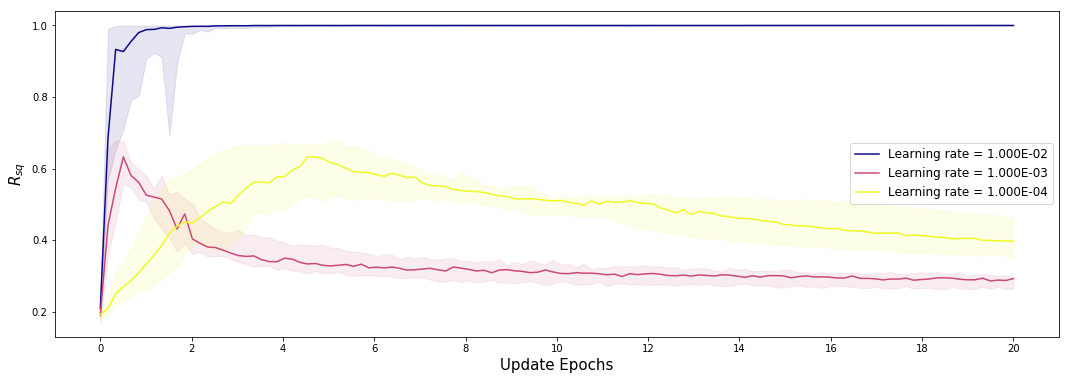
\includegraphics[width=\myWidth]{img/Sec5/sim1/dynamics_e20}
\caption[The dynamics of VNI $R_{sq}$ of the output layer.]
{
The dynamics of VNI $R_{sq}$ of the output layer.
The training is performed on the MNIST dataset 20 times, and then we evaluate the quartiles of the output VNI $R_{sq}$
for different learning rates.
Severe intensification of VNI (increases to 1 ) may occur as shown by the blue line which is trained with the learning rate of $10^{-2}$.
Otherwise VNI rises initially, and then decreases to a value which is larger than the initial VNI.
%It shows that overall, the correlation of each hidden layer is intensified during the back-propagation training. For large learning rate, the output VNI $R_{sq}$ severely increases to 1.
}
\label{fig:sec5_sim1}
\end{figure}


% \begin{figure}
\centering
\newcommand{\myWidth}{0.95\textwidth}
\begin{subfigure}{\myWidth}
  \centering
  \caption{Initial}
  \adjincludegraphics[width=1.0\linewidth,trim={0 0 0 0.8cm},clip]{"Hard-tanh[0]"}
  \label{fig:sec5_sim2_a}
\end{subfigure}%

\begin{subfigure}{\myWidth}
  \centering
  \caption{After 5 updates}
  \adjincludegraphics[width=1.0\linewidth,trim={0 0 0 0.8cm},clip]{"Hard-tanh[5]"}
  \label{fig:sec5_sim2_b}
\end{subfigure}%

\begin{subfigure}{\myWidth}
  \centering
  \caption{After 10 updates}
  \adjincludegraphics[width=1.0\linewidth,trim={0 0 0 0.8cm},clip]{"Hard-tanh[10]"}
  \label{fig:sec5_sim2_c}
\end{subfigure}%
\caption[The averages of squared correlation coefficients $\rho_{ij}^2$ over 50 runs.]
{The averages of squared correlation coefficients $\rho_{ij}^2$ over 50 runs.
It presents that overall, the correlation of each hidden layer are highly intensified.}
\label{fig:sec5_sim2}
\end{figure}



\chapter{Comparison with exploding/vanishing gradients} \label{compare}

In this section, we explore whether the \textit{vanishing node} phenomenon arises from the problem of  exploding/vanishing gradients. Exploding/vanishing gradients in deep neural networks are a problem regarding the scale of forward-propagated signals and back-propagated gradients that exponentially explode/vanish as the networks grows deeper. We perform a theoretical analysis of exploding/vanishing gradients and show analytically the difference between them.
%it and the \textit{vanishing node} phenomena.


%We will first discuss the exploding/vanishing gradients problem via the theoretical model used in Section \ref{why}. We compare exploding and vanishing gradients problem with vanishing node phenomena analytically. Finally, we provide some numerical results to show the difference between exploding/vanishing gradients problem and vanishing node phenomena.

As in a previous study \cite{xavier}, we use the variances of hidden nodes to evaluate the scales of back-propagated gradients. Consider the model and the assumptions in Section \ref{why} and an additional assumption: the gradient of output layer $\frac{\partial Cost}{\partial \mathbf{x}_L}$ is a zero-mean i.i.d. random (row) vector.
That is, $\mathbb{E}[\mathbf{x}_0{\mathbf{x}_0}^T] = \sigma_x^2\cdot\mathbf{I}$ and $\mathbb{E}\Big[\Big(\frac{\partial Cost}{\partial \mathbf{x}_L}\Big)^T\frac{\partial Cost}{\partial \mathbf{x}_L}\Big] = \sigma_y^2\cdot\mathbf{I}$,
where $\sigma_x^2$ and $\sigma_y^2$ are defined as the variances of the input layer nodes and output layer gradients, respectively.
Consider %the forward and backward end-to-end propagation of variances, that is, 
the variances of the output nodes $Var[\mathbf{x}_L]$ and input layer gradients $Var\Big[\frac{\partial Cost}{\partial \mathbf{x}_0}\Big]$, respectively.
The exploding/vanishing gradients  occur only if the scales of forward and backward propagation exponentially increase or decrease as the depth increases.
This means that the magnitude of the gradients will be bounded if we can prevent the scales of forward and backward propagation from exploding or vanishing. 
%Therefore, we can keep forward and backward end-to-end propagation of variances from exploding or vanishing in order to avoid exploding and vanishing gradients problem.

According to the assumptions in Section \ref{why} and  \eqref{covariance_eqn}, we can approximate the shared scalar variance of all output nodes $Var[\mathbf{x}_L]\in\mathbb{R}$ and the shared scalar variance of all input gradients $Var\Big[\frac{\partial Cost}{\partial \mathbf{x}_0}\Big]\in\mathbb{R}$ as

\begin{equation}
    \begin{aligned}
    Var[\mathbf{x}_L] &=\mathbb{E}[(\mathbf{x}_L-\overline{\mathbf{x}_L})^T(\mathbf{x}_L-\overline{\mathbf{x}_L})]/N
    \approx \mathbb{E}[(\mathbf{Jx}_0)^T\mathbf{Jx}_0]/N\\
    &=\mathbb{E}[tr(\mathbf{J}^T\mathbf{J}\mathbf{x}_0\mathbf{x}_0^T)]/N
    =\sigma_x^2\cdot tr(\mathbf{J}^T\mathbf{J})/N
    \label{xvar_to_trace}
    \end{aligned}
\end{equation}

\begin{equation}
    \begin{aligned}
    Var\Big[\frac{\partial Cost}{\partial \mathbf{x}_0}\Big]
    &=\mathbb{E}\Big[\Big(\frac{\partial Cost}{\partial \mathbf{x}_0}-\overline{\frac{\partial Cost}{\partial \mathbf{x}_0}}\Big)
    \Big(\frac{\partial Cost}{\partial \mathbf{x}_0}-\overline{\frac{\partial Cost}{\partial \mathbf{x}_0}}\Big)^T\Big]\Big/N
    \\
    &= \mathbb{E}\Big[
    \Big(\frac{\partial Cost}{\partial \mathbf{x}_L}\mathbf{J}\Big)
    \Big(\frac{\partial Cost}{\partial \mathbf{x}_L}\mathbf{J}\Big)^T\Big]\Big/N
    =\sigma_y^2\cdot tr(\mathbf{J}^T\mathbf{J})/N,
    \end{aligned}
    \label{yvar_to_trace}
\end{equation}

where the chain rule for back-propagation: $\frac{\partial Cost}{\partial \mathbf{x}_0}=\frac{\partial Cost}{\partial \mathbf{x}_L}\frac{\partial \mathbf{x}_L}{\partial \mathbf{x}_0}=\frac{\partial Cost}{\partial \mathbf{x}_L}\mathbf{J}$ is used, and the shared scalar variance of a vector is the average of the variances of all vector components.
Note that because the product of a row vector and a column vector is a scalar, the product is equal to its trace. Also, it is already known that
$tr(\mathbf{J}^T\mathbf{J})=N\cdot m_1=N\cdot(\sigma_w^2\mu_1)^L$. Thus, we have $Var[\mathbf{x}_L]=\sigma_x^2(\sigma_w^2\mu_1)^L$ and $Var\Big[\frac{\partial Cost}{\partial \mathbf{x}_0}\Big]=\sigma_y^2(\sigma_w^2\mu_1)^L$,
where $\sigma_w^2=N\cdot Var[W_{ij}]$, and $\mu_1$ is the first moment of the nonlinear activation function. It is obvious that the variances of both forward and backward propagation will neither explode nor vanish if and only if $(\sigma_w^2\mu_1)=1$.

For the weight gradient of the hidden layer $l$, the variance can be used to measure the scale distribution. Because $\frac{\partial Cost}{\partial \mathbf{W}_l}
=\mathbf{x}_{l-1}\cdot\frac{\partial Cost}{\partial \mathbf{h}_l}$ and both $\mathbf{x}_{l-1}$ and $\frac{\partial Cost}{\partial \mathbf{h}_l}$ are assumed to be zero-mean, the variance of the weight gradient can be evaluated as

\begin{equation}
    Var\Big[\frac{\partial Cost}{\partial \mathbf{W}_l}\Big]
    =
    Var[\mathbf{x}_{l-1}]\cdot
    Var\Big[\frac{\partial Cost}{\partial \mathbf{h}_l}\Big]
    %=
    %\sigma_x^2(\sigma_w^2\mu_1)^{l-1}\cdot
    %\sigma_y^2(\sigma_w^2\mu_1)^{L-l}
    \approx
    \sigma_x^2\sigma_y^2(\sigma_w^2\mu_1)^{L-1},
    \label{weight_var}
\end{equation}
where we can evaluate $Var[\mathbf{x}_{l-1}]$ and $Var\Big[\frac{\partial Cost}{\partial \mathbf{h}_l}\Big]$ using the results of the forward/backward variance propagation and split the entire network into two sub-networks. One sub-network has the input layer $\mathbf{x}_{0}$ and output layer $\mathbf{x}_{l-1}$, and the other sub-network has the input layer $\mathbf{x}_{l}$ and the output layer $\mathbf{x}_{L}$. Note that \eqref{weight_var} also concludes that if and only if $(\sigma_w^2\mu_1)=1$, the weight gradients will never explode or vanish.

However, \eqref{rsq_moment} shows that VNI ($R_{sq}$) may still accumulate with the network depth even if $(\sigma_w^2\mu_1)=1$. That is, the characteristic of the vanishing nodes becomes evident  when $(\mu_2/\mu_1^2-1-s_1)$ is large, whereas vanishing/exploding gradients occurs when $(\sigma_w^2\mu_1)$ is far from 1. If the network's initialization parameter is appropriately set such that $(\sigma_w^2\mu_1)$ is close to 1, $R_{sq}$ may still accumulate due to the network depth, the activation function, and the weight distribution. Therefore, from \eqref{rsq_moment} and \eqref{weight_var}, it is clear that the problem of vanishing nodes  may occur regardless of  exploding/vanishing gradients.

%In Figure \ref{fig:sec6_theo1}, we provide a schematic diagram for evaluating architectures of deep neural networks. The network depth $L$, the network width $N$, the weight initialization scale $\sigma_w^2$, the moments associated with weight $s_1$ and the moments associated with activation $\mu_k$ are taken into consideration. For the horizontal axis, we use the metric $(\sigma_w^2\mu_1)$ to determine whether a network will explode or vanish when the depth $L$ goes deeper. If a network has $(\sigma_w^2\mu_1)=1$, then its scales of gradients will neither vanish nor explode even if the depth $L$ becomes larger. Otherwise, the further $(\sigma_w^2\mu_1)$ is from $1$, the more severe gradients will exponentially explode/vanish. For the vertical axis, we take $R_{sq}$ as the metric. From \eqref{rsq_moment}, we know that $R_{sq}$ is decided by $L$, $N$, $\mu_k$ and $s_1$. If $R_{sq}$ can reach exactly $1/N$, then by \eqref{rsq_moment}, we can show  that correlations of output layer nodes will never accumulate even if the depth $L$ increases. Therefore by Figure \ref{fig:sec6_theo1}, we can determine whether a neural network with specific parameters will suffer from exploding/vanishing gradients and vanishing nodes or not.

% For example in previous works on ultra-deep neural networks, \cite{mft:cnn} chose an activation function that has $\mu_2/\mu_1^2\approx1$ and initialized the weights via appropriately-scaled orthogonal matrices (\cite{mft:linear}) which have $s_1=0$  (from \cite{mft:sigmoid}) and $(\sigma_w^2\mu_1)=1$. Hence the VNI $R_{sq}$ of the network will reach $1/N$, which will not accumulate as the depth $L$ increases according to \eqref{rsq_eigen}. The parameter setting of the network is located at the intersection of vertical and horizontal dashed line in Figure \ref{fig:sec6_theo1}, and thus the network does not suffer from vanishing/exploding gradients and vanishing nodes.


% \begin{figure}
\centering
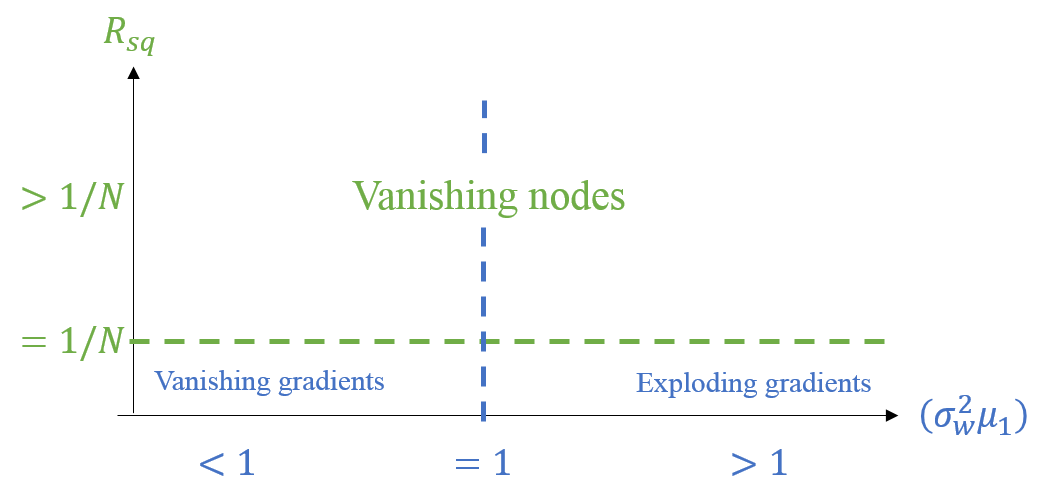
\includegraphics[width=0.7\textwidth]{theo}
\caption{The schematic diagram for deep neural network architectures. To avoid the network from exploding/vanishing gradients and vanishing nodes as the network depth $L$ goes deeper, the best network setting is located at the intersection of vertical and horizontal dashed line.}
\label{fig:sec6_theo1}
\setlength{\belowcaptionskip}{-10pt}
\end{figure}


% According to \eqref{rsq_eigen}, if $R_{sq}$ gets larger, then $m_2$ is also larger compared to $m_1^2$. Recall that $m_i$ is the $i$-th moment of eigenvalues of $\mathbf{JJ}^T$, so the variance of eigenvalues of $\mathbf{JJ}^T$ is $m_2-m_1^2$. Also, eigenvalues of $\mathbf{JJ}^T$ is equivalent to the squared singular values of $\mathbf{J}$. Thus, if the variance of eigenvalues of $\mathbf{JJ}^T$ is too big, the Jacobian $\mathbf{J}$ will become ill-conditioned. Therefore, we can relate $R_{sq}$ to the condition number of Jacobian $\mathbf{J}$, and thus we can link the vanishing node problem to the ill-conditioned Jacobian, which is emphasized in previous works (\cite{mft:sigmoid, mft:spectral, mft:linear}).

% Moreover, \textit{dynamical isometry}, a stronger condition for deep neural networks, is described as "\textit{all} singular values of the Jacobian concentrate near 1" by \cite{mft:sigmoid, mft:linear}. That is, if \textit{dynamical isometry} is achieved, then the variance of singular values of the input-output Jacobian will approach nearly zero, which implies $m_2-m_1^2\approx 0$. Therefore, the $R_{sq}$ will also remain nearly $1/N$ even at a large depth $L$.

% Therefore, we can say that dynamical isometry is not only related to the \textit{learning speed} (\cite{mft:linear}), but also linked to the node correlation $R_{sq}$, which is closely connected with the \textit{learning capability} and the \textit{representation power} of a deep neural network.


%% Below are our numerical results about layer-wise forward and backward variances. As the simulation we have performed in Section 5, we can see that the variances are neither exploding nor vanishing though the nodes in the network are already highly correlated.

% \begin{figure}
    \begin{minipage}[c]{0.67\textwidth}
        \includegraphics[width=\textwidth]{"NodeHistogram"}
    \end{minipage}\hfill
    \begin{minipage}[c]{0.3\textwidth}
        \caption{To show that node vanishing is not arise from gradients exploding or vanishing, we plot histograms of hidden nodes of the updated network in figure \ref{fig:sec5_sim2}. We can observe that the scales of hidden nodes are neither vanishing nor exploding.}
        \label{fig:sec6_sim1}
    \end{minipage}
\end{figure}


\chapter{Experiments} \label{experiments}

\begin{figure}
\centering
\newcommand{\myWidth}{0.4\textwidth}
\newcommand{\myspace}{\hspace{3mm}}
\begin{subfigure}{\myWidth}
  \centering
  \caption{Probability of Success (Tanh, Scaled Gaussian Init.)}
  \adjincludegraphics[width=1.0\linewidth,trim={0 0 0 0.65cm},clip]{"s_tanh_normal_sgd"}
  \label{fig:mnist_sim_s1}
\end{subfigure}\myspace%
\begin{subfigure}{\myWidth}
  \centering
  \caption{Probability of Success (ReLU, Scaled Gaussian Init.)}
  \adjincludegraphics[width=1.0\linewidth,trim={0 0 0 0.65cm},clip]{"s_relu_normal_sgd"}
  \label{fig:mnist_sim_s2}
\end{subfigure}\myspace
\begin{subfigure}{8mm}
  \includegraphics[width=\linewidth]{"s_colorbar"}
\end{subfigure}%
\\
\begin{subfigure}{\myWidth}
  \centering
  \caption{Probability of Success (Tanh, Orthogonal Init.)}
  \adjincludegraphics[width=1.0\linewidth,trim={0 0 0 0.65cm},clip]{"s_tanh_orthogonal_sgd"}
  \label{fig:mnist_sim_s3}
\end{subfigure}\myspace
\begin{subfigure}{\myWidth}
  \centering
  \caption{Probability of Success (ReLU, Orthogonal Init.)}
  \adjincludegraphics[width=1.0\linewidth,trim={0 0 0 0.65cm},clip]{"s_relu_orthogonal_sgd"}
  \label{fig:mnist_sim_s4}
\end{subfigure}\myspace
\begin{subfigure}{8mm}
  \includegraphics[width=\linewidth]{"s_colorbar"}
\end{subfigure}%
  % \caption{Final $R_{sq}$ (Tanh, Scaled Gaussian Init.), the initial $R_{sq}=0.304\pm0.210$.}
  % \caption{Final $R_{sq}$ (Tanh, Orthogonal Init.), the initial $R_{sq}=0.031\pm0.000$.}
  % \caption{Final $R_{sq}$ (ReLU, Orthogonal Init.), the initial $R_{sq}=0.788\pm0.239$.}
% Initial $0.304\pm0.210$, $0.031\pm0.000$ and $1$,
% the final VNI $R_{sq}$ of success/failure are $0.299\pm0.091/0.980\pm0.056$, $0.234\pm0.060/0.945\pm0.133$ and $0.424\pm0.199/0.944\pm0.118$ respectively. 
\caption[Probability of successful training for the SGD optimizer.]
{Probability of successful training for different network depth $L$ and learning rate $\alpha$ (the SGD optimizer). The black color denotes zero probability of successful training.
%We observe that the difficulty of training arises when the VNI $R_{sq}$ increases to 1.
%, and that the orthogonal weight initialization can reduce the probability of failure.
}
\label{fig:mnist_sim}
\end{figure}


To empirically explore the effects of the phenomenon of vanishing nodes on the training of deep neural networks, we perform experiments with the training tasks on the MNIST dataset \cite{mnist}. Because the purpose is to focus on the  vanishing nodes, the networks are designed such that vanishing/exploding gradients will never occur; that is, they are initialized with weights ($\sigma_w^2\mu_1=1$).
%MNIST dataset includes 50,000 training images which have 28$\times$28 grey-scaled pixels.
The network is trained with 100 batch size.
%Since the  purpose  is to focus on the  vanishing nodes, which may lead to the insufficient network representation capability  as shown in Figure \ref{fig:sec5_sim1}, 
The number of successful training for total 20 runs is recorded to reflect the influence of vanishing nodes on the training process, which may lead to the insufficient network representation capability  as shown in Figure \ref{fig:sec5_sim1}.
A successful training is considered to occur when the training accuracy exceeds 90\% within 100 epochs. 
%because the experiment purpose  is to observe the probability of vanishing nodes, which may lead to the insufficient network representation capability during the training process as shown in Figure \ref{fig:sec5_sim1}.
The network depth $L$ ranges from $25$ to $500$, and the network width $N$ is set to $500$.
The learning rate $\alpha$ ranges from $10^{-4}$ to $10^{-2}$ with the SGD algorithm.
Both $L$ and $\alpha$ are uniformly distributed on the logarithmic scale.
The experiments are performed on the MXNet framework\cite{mxnet}.
%Notice that we initialize the matrices with $(\sigma_w^2\mu_1) = 1$ to avoid vanishing/exploding gradients problem, and 
%The probability of successful training is estimated with 10 runs for each hyperparameter setting.

%The probabilities of successful training for (Tanh/ReLU) activation and (Scaled-Gaussian/Orthogonal from \cite{mft:linear}) weights initialization are presented in Figure \ref{fig:mnist_sim}. It shows that a fail training occurs when the depth $L$ and the learning rate $\alpha$ is large, and we observe that the correspond $R_{sq}$ of failed cases increase to $1$, which implies that the vanishing nodes problem is \textbf{the main reason} making the training fails. Similar results can be obtained with different weight initializations (e.g. scaled Uniform) and optimization methods (e.g. SGD+Momentum with coeff. $=0.9$, Adam, RMSProp). Moreover, the (orthogonal + tanh) can reduce the probability for $R_{sq}$ raising to 1 (in Fig. \ref{fig:mnist_sim_s2}), while (scaled-Gaussian + tanh in Fig. \ref{fig:mnist_sim_s1}), (orthogonal + ReLU in Fig. \ref{fig:mnist_sim_s3}) and (scaled-Gaussian + ReLU) cannot. It means that the probability of fail training can be reduced if the VNI evaluated in \eqref{rsq_moment} is close to $1/N$.

Figure \ref{fig:mnist_sim} shows the results of two different activation functions (Tanh/ReLU) with two different weight initializations (scaled-Gaussian/orthogonal from \cite{mft:linear}). When a network with tanh activation functions is initialized with orthogonal weights, the term of  $(\mu_2/\mu_1^2-1-s_1)$ in \eqref{rsq_moment} becomes zero. Therefore, its $R_{sq}$ will be the minimum value ($1/N$) and will not depend on the network depth. For the other network parameters, $(\mu_2/\mu_1^2-1-s_1) $ will not equal zero, and $R_{sq}$ still depends on the network depth. The experimental results show the likelihood of a failed training is high when the depth $L$ and the learning rate are large. In addition, the corresponding $R_{sq}$ of failed cases becomes nearly $1$, which causes a lack of the network representation power.
It implies that the vanishing nodes problem is \textbf{the main reason} that the training fails. A comparison of Figure \ref{fig:mnist_sim_s3} with the other three results shows clearly that the networks with the minimum $R_{sq}$ value have the highest successful training probability.

Shallow network architectures can tolerate a greater learning rate, which is why the vanishing node problem has been ignored in many networks with small depth. In a deep network, the learning rate should be set to small value to prevent $R_{sq}$ from increasing to 1. The experimental results of various training hyperparameters (Momentum, %Batch Normalization,
Adam, RMSProp) are reported in the supplementary material due to space limitations. Also, if more efficient optimization methods (e.g. Adam, RMSProp) are used, the feasible learning rate should become smaller. The scale of the feasible learning rate for RMSProp and Adam should be roughly $10^2$ smaller than that for SGD, and that for SGD+Momentum (with momentum $=0.9$) optimization should be about $10^{0.5}$ smaller.
The reason why the behavior of $R_{sq}$ is effected by learning rates $\alpha$ remain unexplained, suggesting further investigations to better understand the relationship between learning rates and the dynamics of $R_{sq}$
A high learning rate will cause $R_{sq}$ to be severely intensified to nearly 1, and the representation capability of the network will be reduced, which is \textbf{the main reason} that the training fails.
Further analyses of the experiments are provided in the supplementary material.

\chapter{Conclusion} \label{conclusion}

The phenomenon of \textit{vanishing nodes} 
is investigated as another challenge when training deep networks.
Like the vanishing/exploding gradients problem, vanishing nodes also make training deep networks
difficult.
The hidden nodes in a deep neural network become more correlated as the network depth increases,
so the similarity between the hidden nodes increases.
Because similarity between nodes results in redundancy, the effective number of hidden nodes in a
network decreases.
This phenomenon is called\textit{"vanishing nodes"}.

To measure the degree of vanishing nodes, the \textit{Vanishing Nodes Indicator (VNI)} is proposed.
It is shown theoretically that the VNI is proportional to the network depth and inversely proportional
to the network width, which is consistent with the experimental results.
Via this theoretical tool,
we proof that the representation power of a network vanishes as the VNI goes to 1.
The effective number of nodes goes to 1 as when the VNI equals to 1, which is called
the "\textit{network collapsing}".
Also, we show that for a non-orthogonal initialized network, the VNI increases as the network
depth gets larger, and it asymptotically goes to 1 as the network depth tends to infinity.
That is, the network collapses when we consider a very deep feed-forward neural network.

However, if weight matrices are initialized with orthogonal distribution, or if a residual-like
architecture is applied, then the network will not collapse at a large depth.
We show theoretically that orthogonal weight can have small VNI at initial, and that
the network with identity shortcut connection is closer to the orthogonality.
Numerical simulations are also performed on different activation functions, weight initializations
and network architectures, which have a consistent result with our derivation.
Both theoretical and numerical results suggest that the weight initialization and the architecture
of a network determine its trainable depth.
Orthogonal weight initialization and residual-like architecture, from this point of view, are
relatively better for training a very deep neural network.

Moreover, we explore the difference between vanishing/exploding gradients and vanishing nodes,
and suggest a criterion to predict the occurrence of two problems by the network depth,
the network width, the activation, and the weight initialization. 
Finally, experimental results show that vanishing/exploding gradients and vanishing nodes are two
different challenges that make training deep neural networks difficult. 
%have demonstrated that the back-propagation training of networks intensifies the correlation between hidden nodes.


\appendix

\backmatter

\addcontentsline{toc}{chapter}{\bibname}
\bibliographystyle{abbrv}

% Your bibliography goes here
\bibliography{thesis}

\end{document}
